% Autor: Manuel Lippert
% Physikalisches Praktikum

% Main-Datei für die Auswertung in TeX

% Struktur:
% Jedes Kapitel hat einen Input-File. Um Merge-Konflikte zu verhindern wird angeraten für jede 
% Datei eine eigene Tex Datei zu machen und sie im jeweiligen Kapitel zu importieren. Die in
% Input-Struktur dient zur besseren Übersicht und für mögliche Ordner, welche hier vorhanden sind. Die Zahlen vor den 
% Ordner dient zur Ordnung der einzelnen tex-Files nach Kapiteln


% Packages
\documentclass[paper=a4,bibliography=totoc,BCOR=10mm,numbers=noenddot,fontsize=11pt,headsepline]{scrreprt}              
                 
\usepackage[ngerman]{babel}
\usepackage[T1]{fontenc}
\usepackage[latin1, utf8]{inputenc} %ä, ö, ü inbegriffen
\usepackage[babel,german=quotes]{csquotes} %For Quotes
\usepackage{lmodern}
\usepackage{graphicx}
\usepackage{nicefrac}
\usepackage{fancyvrb}
\usepackage{amsmath,amssymb,amstext}
\usepackage{siunitx}
\usepackage{url}
\usepackage[numbers]{natbib}
\usepackage{microtype}
\usepackage[format=plain]{caption}
\usepackage{physics}
\usepackage{titleref} 

% Zusätzliche Packages
\usepackage{geometry} % Verändert Seitengeometrie
\usepackage{anyfontsize} % Alle Schriftgrößen möglich machen
\usepackage[table]{xcolor} % Farbliche Gestaltung Tabellen
\usepackage{ifthen} % Für kompliziertere tex-Files
\usepackage[absolute,overlay]{textpos} %Textboxen
\usepackage{amsfonts} % Schriftarten
\usepackage{xstring} % Stringoperationen
\usepackage{tikz} % Zeichnungen
\usepackage{pdfpages} % Import von pdfs (Protokolle)
\usepackage{hyperref} % Verlinkungen im Dokument
\usepackage{makecell}
\usepackage{subcaption}

% Abschnittseinrückung und -abstand
% Die folgenden Zeilen sollen möglichst nicht verändert werden
\parindent 0.0cm
\parskip 0.8ex plus 0.5ex minus 0.5ex

% Anzahl und Größe von Gleitobjekten
% maximal 2 Objekte oben und unten
% erlaubt auch größere Bilder, welche die ganze Seite benötigen
% Die folgenden Zeilen sollen möglichst nicht verändert werden
\setcounter{bottomnumber}{2}
\setcounter{topnumber}{2}
\renewcommand{\bottomfraction}{1.}
\renewcommand{\topfraction}{1.}
\renewcommand{\textfraction}{0.}

%\sc und \bc veraltet. Daher: (20.09.2018)
\DeclareOldFontCommand{\sc}{\normalfont\scshape}{\@nomath\sc}
\DeclareOldFontCommand{\bf}{\normalfont\scshape}{\textbf}

% Verschiedenes
\pagestyle{headings}          % Der Seitenstil sollte möglichst nicht verändert werden
\graphicspath{{./Bilder/}}    % Der Pfad für die Abbildungen Abbildungen wird gesetzt
\VerbatimFootnotes            % \verb etc. auch in \footnotes mφglich

% Funktionen
\newcommand\tab[1][1cm]{\hspace*{#1}}
\newcommand{\vect}[1]{\boldsymbol{\mathbf{#1}}}
\newcolumntype{g}{>{\columncolor[rgb]{ .741,  .843,  .933}}l}
% Tiefgestellte Zahlen nicht kursiv
\catcode`_=\active
\newcommand_[1]{\ensuremath{\sb{\mathrm{#1}}}}

\begin{document}

    \nonfrenchspacing

    % 0. Kapitel Cover
    % 0. Cover

% Hier sind nur die Variablen und der Abschnitt Informationen (unten) zu bearbeiten der REst läuft automatisch ab (z.b Farbenänderung)

% Noch abänderbar nur ein Vorschlag
\newgeometry{top=30mm, bottom=20mm, inner=20mm, outer=20mm}
\thispagestyle{empty}

% Colors (Notability Colors)
\definecolor{Notablue}{HTML}{3498DB}		
\definecolor{Notared}{HTML}{CF366C}			
\definecolor{Notagreen}{HTML}{19B092}		
\definecolor{Notaorange}{HTML}{FA9D00}		
\definecolor{Notagrey}{HTML}{969696}		
\definecolor{Notalavendel}{HTML}{9DBBD8}	

% Boolean by default false. Für Absatz in der Überschrift
\newboolean{twoRows}
\newboolean{symbol}

% Funktions
\makeatletter
   \def\vhrulefill#1{\leavevmode\leaders\hrule\@height#1\hfill \kern\z@}
\makeatother
\newcommand*\ruleline[1]{\par\noindent\raisebox{.8ex}{\makebox[\linewidth]{\vhrulefill{\linethickness}\hspace{1ex}\raisebox{-.8ex}{#1}\hspace{1ex}\vhrulefill{\linethickness}}}}

% Variables
\def\schriftgrosse{50}
\def\linethickness{1,5pt}

\def\farbe{black}
\def\fach{PPBphys2}
\def\name{Manuel Lippert - Paul Schwanitz}
\def\titel{Rasterelektronen- \\[0,5cm] mikroskop} % Absatz mit \\[0,5cm]; u = Übung, k = Klausur; s = Skript, e = Ergebnis
\def\bottom{WS2021/22}
\def\datum{13.09.2021}
\def\platz{NWII | 2.1.00.267}
\def\betreuer{Inga Elvers}

\def\teilnehmerm{Manuel Lippert}
\def\emailm{Manuel.Lippert@uni-bayreuth.de}
\def\teilnehmerp{Paul Schwanitz}
\def\emailp{Paul.Schwanitz@uni-bayreuth.de}

%\def\auswertp{}
%\def\messp{}
%\def\protop{}

\def\groupnr{11}

\begin{titlepage}
			
	\centering
	{\LARGE \sffamily {\textbf{\bottom}\par}}
	\vspace{2,5cm}
    {\fontsize{30}{0}\sffamily\ruleline{\textcolor{\farbe}{\textbf{\fach}}}\par}
    \vspace{6cm}
	{\Large\sffamily \ruleline{\name}\par}
		
	\IfSubStr {\titel} {\\[0,5cm]} {\setboolean{twoRows}{true}} {\setboolean{twoRows}{false}}
	
	\ifthenelse{\boolean{twoRows}}
		{
			\begin{textblock*}{21cm}(0cm,8,5cm) % {block width} (coords), centered		
				{\fontsize{\schriftgrosse}{0}\sffamily\textcolor{\farbe}{\textbf{\titel}}\par}
			\end{textblock*}
		}
		{
			\begin{textblock*}{21cm}(0cm,9cm) % {block width} (coords), centered		
				{\fontsize{\schriftgrosse}{0}\sffamily\textcolor{\farbe}{\textbf{\titel}}\par}
			\end{textblock*} 
		}
	
	% Choose Logo
	\ifthenelse {\equal{\farbe}{Notared}} {\def\logo{Bilder/Logo/UniBTNotared}}
		{\ifthenelse {\equal{\farbe}{Notagreen}} {\def\logo{Bilder/Logo/UniBTNotagreen}}
			{\ifthenelse {\equal{\farbe}{Notablue}} {\def\logo{Bilder/Logo/UniBTNotablue}}
				{\ifthenelse {\equal{\farbe}{Notaorange}} {\def\logo{Bilder/Logo/UniBTNotaorange}}
					{\ifthenelse {\equal{\farbe}{Notagrey}} {\def\logo{Bilder/Logo/UniBTNotagrey}}
						{\ifthenelse {\equal{\farbe}{Notalavendel}} {\def\logo{Bilder/Logo/UniBTNotalavendel}}	
							{\ifthenelse {\equal{\farbe}{black}} {\def\logo{Bilder/Logo/UniBT}}	
								{\def\logo{noLogo}}
							}
						}
					}
				}
			}
		}	

	\IfSubStr{\logo}{noLogo}{\setboolean{symbol}{false}}{\setboolean{symbol}{true}}
	
	% Gruppe
	\vspace{10cm}
	{\large\sffamily{Gruppe \groupnr}}
	
	%Logo
	\vfill

	\ifthenelse{\boolean{symbol}}
		{
			\begin{figure}[h]
			\begin{center}
				
				\includegraphics[width=2cm]{\logo}
				
			\end{center}
			\end{figure}
		}
	
\end{titlepage}

\restoregeometry

% Information
\chapter*{Informationen}
\label{chap:info}

\begin{tabular}{l l}

	{\textbf{Versuchstag}} \hspace{1cm} & \hspace{1cm} {\datum}\\[0,2cm]
	{\textbf{Versuchsplatz}} \hspace{1cm} & \hspace{1cm} {\platz}\\[0,2cm]
	{\textbf{Betreuer}} \hspace{1cm} & \hspace{1cm} {\betreuer}\\[1,2cm]
	{\textbf{Gruppen Nr.}} \hspace{1cm} & \hspace{1cm} {\groupnr}\\[0.2cm]
	% Für Fortgeschittenenen Praktikum
	{\textbf{Teilnehmer}} \hspace{1cm} & \hspace{1cm} {\teilnehmerm~(\emailm)}\\[0.2cm]
						  \hspace{1cm} & \hspace{1cm} {\teilnehmerp~(\emailp)}\\[0.2cm]
	% Für Grundpraktikum
	%{\textbf{Auswertperson}} \hspace{1cm} & \hspace{1cm} {\auswertp}\\[0.2cm]
	%{\textbf{Messperson}} \hspace{1cm} & \hspace{1cm} {\messp}\\[0.2cm]
	%{\textbf{Protokollperson}} \hspace{1cm} & \hspace{1cm} {\protop}\\[0.2cm]

\end{tabular}

    \thispagestyle{empty}
    \cleardoublepage
    \tableofcontents
    \cleardoublepage

    % 1. Kapitel Einleitung
    \chapter{Introduction}
Hyperfine structures are defined by small shifts in degenerate energy levels, so basically it's the 
smallest energy distance in atoms, molecules, or ions. 
The hyperfine structure arises from the energy of the nuclear magnetic dipole moment interacting with the magnetic field
 and the nuclear electric quadrupole moment in the electric field, at least in atoms.\\
One Possibility to measure such small distances as the hyperfine structures is the Doppler free spectroscopy
which we will use in our experiment. 
During our experiment we will investigate rubidium and its hyperfine structure in more detail.\\
Rubidium is the chemical element with the symbol Rb and atomic number 37, so it’s a alkali metal. 
Natural rubidium comprises two isotopes: \ce{^{85}Rb} (72\%, stable), and 28\% is slightly radioactive \ce{^{87}Rb}.
Furthermore, rubidium can be handled as one electron system, which is useful for the following data analysis. 
However, in this experiment we will have a closer look at the fine and hyperfine structure of 
\ce{^{87}Rb} and \ce{^{85}Rb}, as well as the transition energy and the ratio its isotopes. 


    % 2.Kapitel Theorie
    % 2. Fragen zur Vorbereitung

\chapter{Theoretischer Hintergrund}
\label{chap:theo}

% Text

% Input der Teilaufgaben je nach Produktion der Nebendateien ohne Ordner

\section{Rauschen}

Dieser Abschnitt soll einen groben Überblick über die verschiedenen Arten von Rauschen und ihre Ursachen liefern.

\subsection{Thermisches Rauschen}
Das thermische Rauschen wird von den statistischen Bewegungen der freien Ladungsträger, meist Elektronen, verursacht. Das thermische Rauschen ist weiterhin von der Frequenz unabhängig, weshalb es oft als weißes Rauschen bezeichnet wird.
Die Rauschspannung $u_R$, an einem Widerstand $R$, kann mit folgender Formel berechnet werden: 
\begin{align}
    u_R = \sqrt{4kTRB} \qquad \text{mit} \quad B = f_{max} - f_{min}
    \label{eq:thR}
\end{align}
Wobei T die absolute Temperatur ist und k die Boltzmannkonstante. B bezeichnet die Bandbreite des Messgerätes. Da es sich um statistische Schwankungen handelt, ergibt eine Mittelung von $u_R$ über die Zeit Null.\\
Aus obiger Formel \ref{eq:thR} kann durch die Division durch R eine Formel für die Rauschleistung hergeleitet werden.
\begin{align}
    P_R = 4kTB
\end{align}
Es geht klar hervor, dass die Rauschleistung nur von Temperatur und Frequenz abhängt. Somit wäre es also theoretisch möglich das thermische Rauschen, durch Kühlung des Versuchsaufbaus auf den absoluten Nullpunkt, abzustellen. Dies ist jedoch nicht praktikabel, da es mit enormen Kosten und Aufwand verbunden wäre \citep{VA}.

\subsection{Schrotrauschen}
Wie das thermische Rauschen ist auch das Schrotrauschen ein statisches und von der Frequenz unabhängiges Rauschen, weshalb es ebenfalls ein weißes Rauschen ist. Die Ursache ist jedoch die Quantelung der elektrischen Ladung, welche sich ebenfalls stochastisch bewegen und somit das Schrotrauschen verursachen. Der Effektivwert des Rauschstroms $i_R$ kann durch folgende Formel ausgedrückt werden:
\begin{align}
    i_R^2 = 2eIB
\end{align}
Wobei B wieder die Bandbreite des Messgerätes ist, e die Elektronenladung und I der fließende Gleichstrom.
Für die Rauschleistung $P_R$, über einen Übergang mit Widerstand $R$, gilt: 
\begin{align}
    P_R = i_R^2 R = 2eIRB
\end{align}
Aus dieser Formel ist ableitbar, dass das Schrotrauschen durch die Erniedrigung des Gleichstroms, der durch den Übergang fließt, erreicht werden kann \citep{VA}.

\subsection{Funkelrauschen}
Durch Störstellen im Material kann es zu Funkelrauschen kommen, welches mit zunehmender Frequenz abnimmt. Deshalb wird es auch als $\frac{1}{f}$ Rauschen bezeichnet. Abhilfe schafft hier, die Messungen bei hohen Frequenzen durchzuführen \citep{VA}.

\newpage
\section{Umwelteinflüsse}
\label{sec:umwelt}
Häufig ist bei Messungen jedoch nicht nur Rauschen ein Problem, sondern störende Umwelteinflüsse. Unsere Umwelt ist voll von Störquellen wie elektromagnetischen Wellen, beispielsweise von Radiosendern, welche die Messungen verfälschen, da Kabel im Versuchsaufbau für diese als Antenne fungieren können. Eines der stärksten Störeinflüsse ist wohl das Netzbrummen, was durch die öffentliche Stromversorgung bei 50 Hz verursacht wird. Ebenso können diverse elektrische Geräte wie Elektromotoren oder alte Röhrenmonitore Störungen verursachen \citep{VA}.\\

Um die Einstrahlung von störenden elektromagnetischen Wellen zu vermeiden ist eine gute Abschirmung von diesen vonnöten.
Darum werden die Messgeräte abgeschirmt und Koaxialkabel verwendet. Ein Koaxialkabel besteht aus einem Draht, welche von einer Isolierschicht umgeben ist, welche wiederum durch ein Drahtgeflecht umgeben ist. Als letztes umgibt das Kabel noch eine weitere Isolierung. Der Aufbau wird in Abbildung \ref{fig:Koaxialkabel} veranschaulicht. Das Drahtgeflecht dient hierbei als Schirm und verhindert somit die Einstrahlung von Störeinflüssen. Des Weiteren dient der Schirm auch dazu, um ein gemeinsames Erdpotential bereitzustellen, was eine Störung durch Erdschleifen verhindert. Erdschleifen werden im nächsten Kapitel genauer erklärt.

\begin{figure}[h]
    \centering
    \includegraphics[width=\textwidth]{KoaxialKabel.jpeg}
    \caption{Aufbau eines Koaxialkabels und Schaltsymbol (unten rechts) \citep{VA}}
    \label{fig:Koaxialkabel}
\end{figure}

\newpage
\section{Erdschleifen}
Im vorherigen Abschnitt wurde bereits der Begriff Erdschleifen genannt, welcher nun genauer erklärt werden soll. Wenn die Abschirmungen verschiedener Apparaturen nicht miteinander verbunden sind, sondern jede einzeln geerdet ist, dann existieren dennoch kleine Potenzialunterschiede, die elektrostatisch in das System eingekoppelt werden und somit Störungen verursachen. Um Erdschleifen zu vermeiden, sollten alle Abschirmungen verbunden sein und an einem einzigen Erdungspunkt geerdet werden \citep{VA}. In Abbildung \ref{fig:Erdschleife} wird dies schematisch dargestellt.
\begin{figure}[h]
    \centering
    \begin{subfigure}{0.45\textwidth}
        \centering
        \includegraphics[width=\textwidth]{Erdschleife.jpeg}
        \caption{Falsche Erdung \citep{VA}}
    \end{subfigure}
    \hfill 
    \begin{subfigure}{0.45\textwidth}
        \centering
        \includegraphics[width=\textwidth]{keineErdschleife.jpeg}
        \caption{Richtige Erdung \citep{VA}}
    \end{subfigure}
    \caption{Beispiele für falsche und richtige Erdung}
    \label{fig:Erdschleife}
\end{figure}
% Teilaufgabe 11
\newpage
\section{Möglichkeiten der Signal-Rausch Verbesserung}
\label{sec:verbesserung}
Dieser Abschnitt behandelt die Methoden zur Signal/Rausch-Verbesserung und dessen Umsetzung.
\subsection{Filter}
\label{sub:filter}
Eine Möglichkeit zur Signal/Rausch-Verbesserung ist der Einsatz eines Filters. Die Aufgabe des Filters ist hierbei die Unterdrückung bestimmter Frequenzen. Dabei ist zu beachten, dass das Signal bei einer anderen Frequenz auftritt als das Rauschen, sonst würden man nämlich das Signal mit filtern. Bei der Filterung wird die Bandbreite das Rauschen stark reduziert (Zu sehen an Gleichung (2.1) und (2.3)), aber auch Störstrahlen aus der Umgebung werden minimiert \citep{VA}.
\subsection*{Filtertypen}
\begin{itemize}
    \item[1)]\textbf{Tiefpass}\\
    Ein Tiefpassfilter filtert Frequenzen \textbf{oberhalb} der Grenzfrequenz heraus und lassen Frequenzen unterhalb nahezu ungedämpft durch. Die Grenzfrequenz ist dadurch charakterisiert, dass das Ausgangssignal zu dieser Frequenz um 3dB kleiner ist (ab dort beginnt der Durchlassbereich) \citep{electronik}.
    \item[2)]\textbf{Hochpass}\\
    Ein Hochpassfilter filtert Frequenzen \textbf{unterhalb} der Grenzfrequenz heraus und lassen Frequenzen oberhalb nahezu ungedämpft durch. Ein Hochpassfilter ist das Gegenstück zum Tiefpassfilter \citep{electronik}. Ein Hochpassfilter kann dazu verwendet werden, die 50Hz Brummspannung aus dem Messsignal zu filtern \citep{VA}.
    \item[3)]\textbf{Bandpass}\\
    Ein Bandpass sperrt Frequenzen \textbf{unter- und oberhalb} eines definierten Frequenzbandes. Das Frequenzband ist durch die 3dB-Bandbreite um die Mittenfrequenz charakterisiert. Diese Art des Filters ist eine Reihenschaltung aus Tiefpass- und Hochpassfilter und die Bandbreite wird durch die Grenzfrequenzen der jeweiligen Filter festgelegt \citep{electronik}. Der Bandpass findet heirbei Einsatz bei der Filterung von breitbandigen Rauschen \citep{VA}.
    \item[4)]\textbf{Bandsperre/Notch-Filter}\\
    Ein Bandsperre sperrt einen schmalen Frequenzbereich innerhalb eines breiten Frequenzbandes und kann wie das Gegenstück zu einem Bandpass angesehen werden \citep{electronik}.
\end{itemize}
In Abbildung \ref{image:verlauf} ist der generelle Verlauf der jeweiligen Filtertypen im Frequenzbereich dargestellt.
\newpage
\begin{center}
    \includegraphics[scale=0.3]{VerlaufFilter.png}
    \captionof{figure}{Verlauf der jeweiligen Filtertypen im Frequenzbereich \citep{grafikQuelle}}
    \label{image:verlauf}
\end{center}
\subsection*{Ordnung eines Filters}
Die Ordnung eines Filters gibt an wie oft ein Filter hintereinander in Reihe geschaltet wurde. Somit wären zwei Tiefpassfilter in Reihe geschaltet ein Tiefpassfilter 2.Ordnung. Je höher die Ordnung eines Filters ist, desto steiler ist die sogenannte Flankensteilheit (Steigung der Flanken in Abbildung \ref{image:verlauf}). Es ist aber zu beachten, dass sich durch die Ordnung die Phase in der Nähe der Grenzfrequenz verändern kann \citep{electronik}.
\subsection*{Arten der Filterimplementierung}
\begin{itemize}
    \item[1)]\textbf{Butterworth-Tiefpassfilter}\\
    Der Butterworth-Tiefpassfilter besitzt einen lagen horizontalen Frequenzgang, welcher erst kurz vor der Grenzfrequenz scharf abknickt. In der Sprungantwort lässt sich ein kräftiges Überschwingen (abhängig von der Ordnung) registrieren \citep{VA}.
    \item[2)]\textbf{Tschebyscheff-Tiefpassfilter}\\
    Ein Tschebyscheff-Tiefpassfilter besitzt oberhalb der Grenzfrequenz einen noch steileren Abfall als der Butterworthfilter, womit das Überschwingen der Sprungantwort im Vergleich noch stärker ist. Im Durchlassbereich verläuft die Verstärkung aber nicht monoton, sondern wellig mit konstanter Amplitude \citep{VA}.
    \item[3)]\textbf{Bessel-Tiefpassfilter}\\
    Der Bessel-Tiefpassfilter besitzt unter der Voraussetzung, dass die Phasenverschiebung in einem bestimmten Frequenzbereich proportional zur Frequenz ist, ein optimales Rechteck-Übertragungsverhalten. Der Frequenzgang knickt aber nicht so stark ein, wie bei den zwei vorher genannten Filter \citep{VA}.
    \item[4)]\textbf{Tschebyscheff-Tiefpass}\\
    Der Tschebyscheff-Tiefpass besitzt nach der Grenzfrequenz einen steilen Knick im Frequenzgang, wodurch auch dieser Filter eine Überschwingung der Sprungantwort aufweist. Dies hat zur Folge, dass der Frequenzgang im Durchlassbereich eine Welligkeit besitzt. Durch Verminderung dieser Welligkeit geht der Tschebyscheff kontinuierlich in den Butterworth über \citep{VA}. 
\end{itemize}

\subsection{Signalmittelung}
\label{sub:mittelung}
Bei stark verrauschten Signalen wird die Signalmittelung verwendet. Zu beachten ist aber, dass die Bandbreiten des Signals und des Rauschens in derselben Größenordnung liegen, was die Anwendung eines Filters ausschließen würde. Eine weitere Voraussetzung ist, dass das Signal wiederholbar und dessen Phase bekannt ist. Bei der Signalmittelung wird das Signal mit Rauschen in $n$ Segmente unterteilt und in $n$ Kanälen gespeichert. Dieser Vorgang wird mehrmals wiederholt und jeder neue Durchgang zum vorhandenen Speicherinhalt addiert, was ein Anwachsen des Signals proportional zu den Wiederholungen verursacht. Beim Rauschen aufgrund seiner statischen Natur wird nur der quadratischen Mittelwert auf das vorhandene Messsignal addiert. Allgemein erhält man für $N$ Wiederholungen eine Signal/Rausch-Verbesserung von $\sqrt{N}$ \citep{VA}. In Abbildung \ref{image:mittelung} wird die erzielte Signal/Rausch-Verbesserung durch ein Vorher-Nachher-Bild gezeigt.
\begin{center}
    \begin{tabular}{c c}
        \includegraphics[scale = 0.3]{Mittelung1.png} &
        \includegraphics[scale = 0.3]{Mittelung2.png}  
    \end{tabular}
    \captionof{figure}{Anwendung Signalmittelung: Links Signalmessung und Rechts Mehrfachmessung \citep{VA}}
    \label{image:mittelung}
\end{center}
\newpage
\subsection{Lock-In Verstärker}
\label{sub:lockin}
Ein Lock-In Verstärker ist ein Detektor zum Auflösen von kleinen Wechselspannungssignalen bis zu ein paar nV. Dabei ist eine akkurate Messung des Signals, welches 1000\,fach stärkeres Rauschen besitzt, möglich. Es kommt dafür eine sogenannte phasensensitive Detektion zum Einsatz, um eine bestimmte Komponente des Signals bei einer bestimmten Referenzfrequenz $f_{r}$ und Phase $\Theta_{r}$ zu bestimmen. Dabei wird Rauschen, welches nicht auf der Referenzfrequenz liegt, herausgefiltert und trägt nicht mehr zum Signal bei.
\subsection*{Phasensensitive Detektion}
Beim Lock-In wird wie oben erwähnt eine Referenzfrequenz benötigt. Diese Frequenz wird meistens durch das Experiment vorgegeben (z.B. Funktionsgenerator) und der Lock-In detektiert die Antwort des Experiments bei dieser Referenzfrequenz. In Abbildung \ref{image:signalRef} sind schematisch die jeweiligen Signale gezeigt. Als Referenzsignal wird eine Rechteckschwingung mit $f_{r}$ verwendet und das Experiment selbst wird von einer Sinusschwingung (Input-Signal) mit Funktion $s(t)=U_{s}\sin(\omega_{r}t + \Theta_{s})$ mit $\omega_{r}=2\pi f_{r}$, Amplitude $U_s$ und Phasenverschiebung $\Theta_{s}$ angeregt. Der Lock-In Verstärker erzeugt dann selbst eine Sinusschwingung mit Frequenz $f_l$ und der Funktion $l(t) = \sin(\omega_{l}t + \Theta_{r})$ mit $\omega_{l}=2\pi f_{l}$ als Signal, das Lock-In-Signal.
\begin{center}
    \includegraphics[scale = 0.25]{SignalLockIn.png}
    \captionof{figure}{Signale bei einem Lock-In Verstärker \citep{lockin}}
    \label{image:signalRef}
\end{center}
Nun multipliziert der Lock-In Verstärker das Input-Signal und das Lock-In-Signal mit einem phasensensitiven Detektor (PSD) oder einem Multiplikator. Daraus folgt mit Anwendung des Additionstheorems des Sinus:
\begin{gather}
    \begin{aligned}
        s_{x} &= s(t)\cdot l(t) = U_{s}\sin(\omega_{r}t + \Theta_{s}) \cdot \sin(\omega_{l}t + \Theta_{r})\\
                &= \frac{U_{s}}{2}\left[\cos((\omega_{r}-\omega_{l}) + (\Theta_s - \Theta_r)) + \cos((\omega_{r}+\omega_{l}) + (\Theta_s + \Theta_r))\right]
    \end{aligned}
\end{gather}
Damit ist das Output-Signal $s_x$ zwei Wechselspannungssignale mit unterschiedlichen Frequenzen. Dieses Signal wird durch einen Tiefpassfilter geschickt, welcher alle Wechselspannungssignale ab der Grenzfrequenz $f_g$ eliminiert. Die Grenzfrequenz $f_g$ wird dabei am Lock-In Verstärker über die Zeitkonstante $\tau$ eingestellt mit der Beziehung: $f_g\sim\frac{1}{\tau}$\\ Wenn $\omega_r = \omega_l$ ist, ist das Signal mit der Differenz der Frequenz ein Gleichspannungssignal und wird somit nicht gefiltert. Der neue PSD Output ist dann:
\begin{gather}
    s_{x} = \frac{U_s}{2} \cos(\Theta_s-\Theta_r) = \frac{U_s}{2} \cos(\Delta\Theta)  
\end{gather}
Bei einem Phasenunterschied von $\Delta\Theta = 0$ lässt sich hierbei das Maximum der Amplitude messen ($\frac{U_s}{2}$) und bei $\Delta\Theta = \frac{\pi}{2}$ misst man überhaupt kein Output-Signal mehr. Solche Lock-In Verstärker mit nur einem PSD werden auch Einphasen-Lock-In genannt. Man kann aber auch ein zweites Lock-In-Signal mit Cosinusschwinung verwenden und dieses mit einem zweiten PSD mit dem Input-Signal multiplizieren. Mit demselben Prozess wie zuvor erhält man die Beziehung:
\begin{gather}
    s_{y} = \frac{U_s}{2} \sin(\Delta\Theta) 
\end{gather} 
Das Output $s_x$ heißt \enquote{in Phase}-Komponente und $s_y$ die \enquote{Quadratur}-Komponente, weil bei $\Delta\Theta = 0$ ist $s_y = 0$ und $s_x$ misst das Input-Signal.\\

Weiterhin kann man mit $s_x$ und $s_y$ wie folgt die Amplitude des Output-Signals bestimmen:
\begin{gather}
    A = (s_x^2 + s_y^2)^{\frac{1}{2}} = \frac{U_s}{2}
\end{gather}
\subsection*{Was wird mit einem Lock-In gemessen?}
Ein Lock-In Verstärker misst aufgrund der Multiplikation mit einer Sinusschwingung (Cosinusschwingung) den ersten Term der Fourier-Reihe des Input-Signals bei der Referenzfrequenz $f_r$. Dabei ist aber zu beachten, dass auch Rauschen, welches bei der Referenzfrequenz auftritt, mit gemessen wird und gegebenenfalls abgezogen werden muss. Dies erkennt man daran, dass das Messsignal am Lock-In Verstärker Schwankungen aufweist.\\ In Abbildung \ref{image:Block} ist zusätzlich der Aufbau des Lock-In Verstärkers dargestellt \citep{lockin}.
\newpage
\begin{center}
    \includegraphics[scale = 0.6]{BLockdiagrammLockIn.png}
    \captionof{figure}{Blockdiagramm Lock-In Verstärker \citep{lockin}}
    \label{image:Block}
\end{center}

\newpage
\section{Leistungspegel}
\label{sec:pegel}
Der Leistungspegel $L_p$ gibt das 10fache logarithmische Verhältnis zwischen Nutzleistung $P$ und Bezugsleistung $P_0$ in \si{\deci\bel} an und ist definiert als:
\begin{gather}
    L_P = 10 \log_{10}\left(\frac{P}{P_0}\right)
    \label{eq:pegel}
\end{gather}
In diesem Versuch ist vom Interesse den Leistungspegel der Spannungen $L_U$ anzugeben. Dafür wird die Formel $P = U \cdot I$ mit dem ohmischen Gesetz $R = \frac{U}{I}$ umgestellt zu $P = \frac{U^2}{R}$ und in Gleichung (\ref{eq:pegel}) eingesetzt. Somit erhält man:
\begin{gather}
    L_U = 10 \log_{10}\left(\frac{U^2}{U_0^2}\right) = 20 \log_{10}\left(\frac{U}{U_0}\right)
    \label{eq:spannungpegel}
\end{gather}
Damit entspricht der Leistungspegel der Spannungen das doppelte des herkömmlich definierten Leistungspegel \citep{electronik}.\\
Um das Verständnis zu vertiefen werden noch einige bestimmte Verhältnisse zu charakteristischen \si{\deci\bel} angegeben:
\begin{center}
    \begin{tabular}{c | c c}
        $L$/dB & $\frac{P}{P_0}$ & $\frac{U}{U_0}$\\
        \hline
        $-n\cdot10$ & $1\cdot10^{-n}$ &  $1\cdot10^{-n/2}$ \\
        -20 & 1/100 & 1/10 \\
        -10 & 1/10 & 1/$\sqrt{10}$ \\
        -6 & 1/4 & 1/2\\
        -3 & 1/2 & 1/$\sqrt{2}$\\
        0 & 1 & 1\\
        3 & 2 & $\sqrt{2}$\\
        6 & 4 & 2\\
        10 & 10 & $\sqrt{10}$ \\
        20 & 100 & 10 \\
        $n\cdot10$ & $1\cdot10^{n}$ &  $1\cdot10^{n/2}$ \\
    \end{tabular}
    \captionof{table}{Leistungspegel und zugehörige Verhältnisse}
    \label{tab:pegel}
\end{center}
In Tabelle \ref{tab:pegel} lässt sich sehr gut die Verdopplungsregel des Leistungspegels erkennen. Dabei steigt der Pegel um 3\,dB an (bei $L_U$ um 6\,dB), wenn man das Verhältnis verdoppelt. Dies hat damit zu tun, dass der 10er-Logarithmus von 2 ungefähr 0.3 ist und dieser mit der Multiplikation von 10 nach der Gleichung (\ref{eq:pegel}) dann 3\,dB ergibt.
\newpage
\section{Theorem von Nyquist}
Das Theorem von Nyquist oder auch Abtasttheorem besagt, dass aus den Abtastwerten das ursprüngliche Signal (kontinuierlich) fehlerfrei rekonstruiert werden kann, wenn die Abtastfrequenz mindestens doppelt so groß ist wie die höchste Signalfrequenz $f_{max}$. 
\begin{gather}
    f \geq 2\cdot f_{max}
\end{gather} 
Die Frequenz $2\cdot f_{max}$ wird als \textit{Nyquist-Frequenz} bezeichnet. Aus dem Abtasttheorem folgt auch, dass das Spektrum des Signals \textit{bandbegrenzt} ist, d.h. das Signal im Spektrum muss ab der maximalen Frequenz $f_{max}$ gleich 0 sein \citep{praktikum}.
\section{Fouriertransformation und Schnelle Fouriertransformation}
Bei einer Fouriertransformation wird ein gegebenes Signal (ggf. eine Funktion) komplett in den Frequenzraum transformiert, dabei wird ein Integral von $-\infty$ bis $\infty$ ausgewertet. Der Rechenaufwand einer Fouriertransformation ist in der Regel in der Praxis sehr hoch, weswegen meist eine Schnelle Fouriertransformation (engl. Fast Fourier Transformation (FFT)) durchgeführt wird. Unter einer FFT versteht man eine effiziente Realisierung der Diskrete Fouriertransformation (DFT), mit der redundante Rechenschritte vermieden werden. Bei einer DFT wird nur ein abgetastetes Signal in den Frequenzraum überführt. Der Rechenaufwand von $N^2$ bei einer DFT verringert sich dann  bei einer FFT zu etwa $N\log_2\left(N\right)$ \citep{praktikum}.
\section{Fourier-Reihe und Effektivspannung}
\label{sec:fourierseries}
\subsection*{Allgemeines zur Fourier-Reihe und Effektivspannungen}
\label{sub:fourierseriesAllgemein}
Eine Fourier-Reihe zerlegt eine gegeben periodische Funktion in ihre jeweiligen Sinus und Cosinusanteile. Die reelle Fourier-Reihe einer bestimmten $T$-periodischen Funktion lässt sich mit den folgenden Formeln berechnen:
\begin{gather}
    f(t) = \frac{a_0}{2} + \sum^{\infty}_{k=1} \left[a_k \sin(k\frac{2\pi}{T} t) +b_k \cos(k\frac{2\pi}{T} t)\right]\\
    a_k = \frac{2}{T} \int^{\frac{T}{2}}_{-\frac{T}{2}} f(t)\cos(k \frac{2\pi}{T} t)dt \tab
    b_k = \frac{2}{T} \int^{\frac{T}{2}}_{-\frac{T}{2}} f(t)\sin(k \frac{2\pi}{T} t)dt
\end{gather}
Dabei sind die Grenzen der Integrale von $-\frac{T}{2}$ bis $\frac{T}{2}$ nicht fest, sie können verschoben werden. Es ist aber wichtig, dass über eine Periode integriert wird in diesem Fall über eine komplette Periodendauer $T$ \citep{praktikum}.\\

Um die effektiven Spannungswerte der jeweiligen Schwingungsform zu bestimmen, bildet man das sogenannte \enquote{Quadratische Mittel}. Dieses ist wie folgt definiert:
\begin{gather}
    U_{eff} = \sqrt{\frac{1}{T}\int^T_0 f(t)^2 dt}
\end{gather}
Hierbei ist es wieder zu erwähnen, dass die Grenzen der Integration nicht fest sind, aber die Integration über eine Periodenlänge erfolgen muss \citep{messtechnik}.\\

Die detaillierteren Berechnungen zu jeder Schwingungsform lassen sich in Anhang \ref{app:Berechnung} nachlesen.

\subsection*{Sinusschwingung}
\label{sub:sinus}
Der Fall der Sinusschwingung ist besonders einfach, da wie vorangegangen erwähnt, die Fourier-Reihe eine periodische Funktion in ihre Sinus und Cosinusanteile zerlegt. Daraus folgt die Fourier-Reihe der Sinusschwingung ist die Sinusschwingung selbst und kann somit trivial angegeben werden als:
\begin{gather}
    \boxed{f(t) = U_0\sin(\frac{2\pi}{T} t)}
\end{gather}
Die Effektivspannungen der Sinusschwingung:
\begin{gather}
    \boxed{U_{eff}=\frac{U_0}{\sqrt{2}}\approx 0,70711 \cdot U_0}
\end{gather}

\subsection*{Rechteckschwingung}
\label{sub:square}
Als Nächstes wird die Fourier-Reihe der Rechteckschwingung bestimmt. Diese hat die Form:
\begin{gather}
    f(t) = 
    \begin{cases}
        +U_0, & 0 \leq t \leq \frac{T}{2} \\
        -U_0, & \frac{T}{2} \leq t \leq T \\
    \end{cases}
\end{gather}
Da die Funktion der Rechteckschwingung punktsymmetrisch zum Ursprung ist, fallen alle Cosinusanteile weg, da $a_k = 0$. Somit muss nur $b_k$ wie folgt berechnet werden:
\begin{gather}
    b_k =
    \begin{cases}
        0, & k~\text{gerade}\\
        \frac{4U_0}{\pi}\frac{1}{k}, & k~\text{ungerade}\\
    \end{cases}
\end{gather} 
Es werden nur noch Terme mit ungeraden $k$ betrachtet und man erhält:
\begin{gather}
    \boxed{f(t) = \frac{4U_0}{\pi} \sum^{\infty}_{k=1} \frac{1}{2k-1} \sin((2k-1)\frac{2\pi}{T}t)}
\end{gather}
Die Effektivspannungen der Rechteckschwingung:
\begin{gather}
    \boxed{U_{eff} = U_0}
\end{gather}
\subsection*{Dreiecksspannung}
\label{sub:triangle}
Als Letztes wollen wir die Dreieckschwingung betrachtet. Die Form dieser ist definiert wie folgt:
\begin{gather}
    f(t) = 
    \begin{cases}
        at, & -\frac{T}{4} \leq t \leq \frac{T}{4} \\
        a\left(\frac{T}{2}-t\right), & \frac{T}{4} \leq t \leq \frac{3T}{4} \\
    \end{cases}
    ~\text{mit}~U_0 = \frac{aT}{4}
\end{gather} 
Die Funktion ist erneut punktsymmetrisch zum Ursprung, wodurch wieder alle $a_k$-Koeffizienten 0 sind. $b_k$ ergibt sich dann durch wie folgt:
\begin{gather}
    b_k =
    \begin{cases}
        0, & k~\text{gerade}\\
        \frac{8U_0}{\pi^2}\frac{(-1)^{k-1}}{k^2}, & k~\text{ungerade}\\
    \end{cases}
\end{gather}
Es werden wieder nur die Terme mit ungeraden $k$ betrachtet. Somit erhält man:
\begin{gather}
    \boxed{f(t) = \frac{8U_0}{\pi^2} \sum^{\infty}_{k=1} \frac{(-1)^{k-1}}{(2k-1)^2} \sin((2k-1)\frac{2\pi}{T}t)}
\end{gather} 
Die Effektivspannungen der Dreieckschwingung:
\begin{gather}
     \boxed{U_{eff} = \frac{U_0}{\sqrt{3}}\approx 0,57735 \cdot U_0}
\end{gather}
\section*{Gemeinsamkeiten von Rechteck und Dreiecksschwingung}
Vergleicht man die Fourierreihe der Rechteck und Dreiecksschwingung erkennt man, dass beide Reihen nur aus Sinusschwingungen bestehen mit den selben Argumenten. Weiterhin ist zu erwähnen, dass die Reihen nur ungerade $k$ besitzen. Die einzigen Unterschiede treten auf bei den Vorfaktoren und den Summenkoeffizienten. Bei den Summenkoeffizienten besitzt die Rechteckschwingung eine $\frac{1}{k}$-Faktor, während die Dreiecksschwingung einen $\frac{1}{k^2}$-Faktor, welcher alterniert, aufweist. Dieser Vergleich zeigt deutlich, dass zwischen den beiden Schwingungsformen in ihrem Aufbau kein großer Unterschied in der Fourierreihe besteht, obwohl die Signal verschiedene Eigenschaften und Formen besitzen.

% etc.

    % 3.Kapitel Protokoll
    
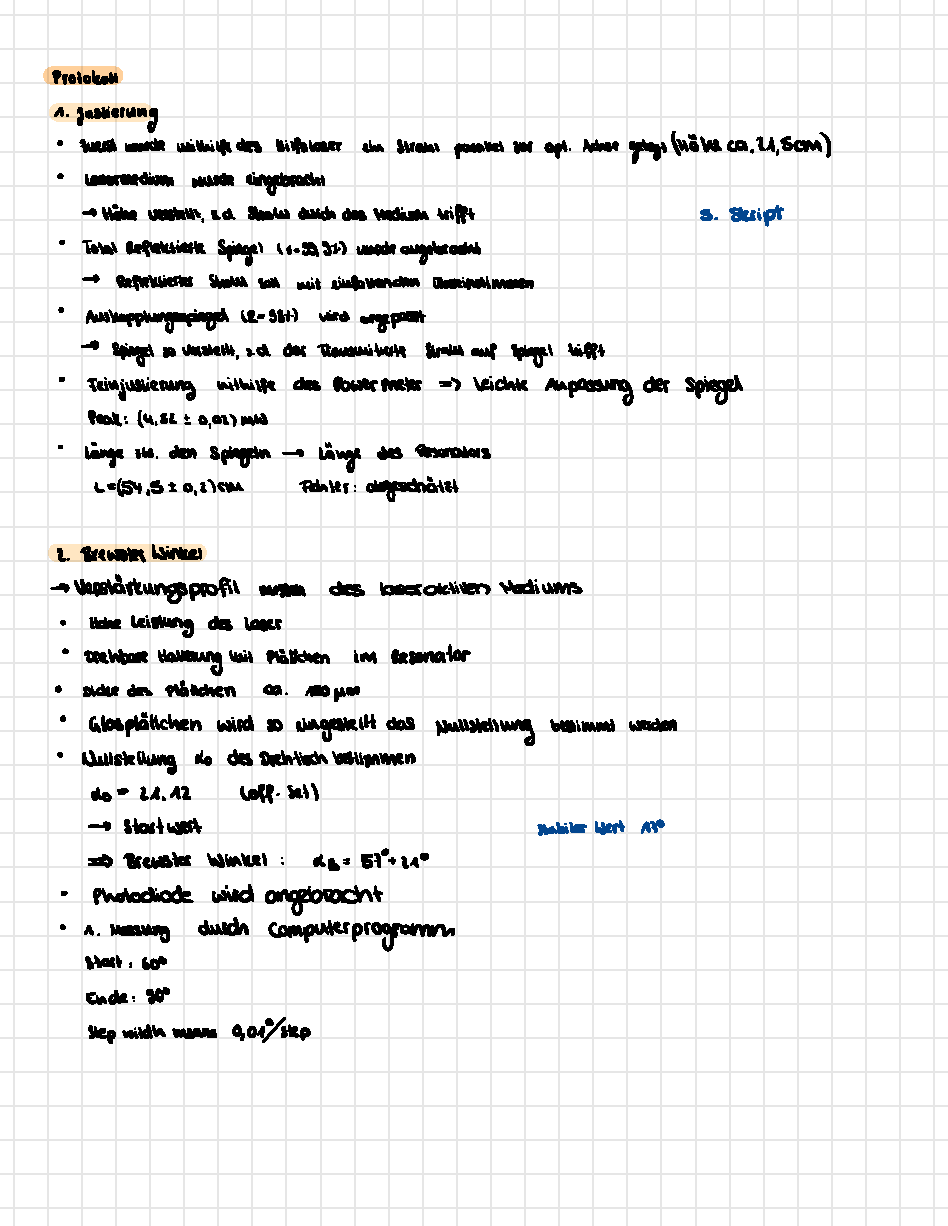
\includepdf[pages=1,landscape = false, offset=0 -25mm, scale=0.71,pagecommand ={\thispagestyle{empty}}\chapter{Protocol}]{Protokoll_Messung/Protokoll.pdf}

\includepdf[pages={2-4},scale=0.8,pagecommand ={\thispagestyle{plain}}]{Protokoll_Messung/Protokoll.pdf}

    % 4.Kapitel Versuchsauswertung
    % 4. Versuchsauswertung

\chapter{Auswertung und Diskussion}
\label{chap:versuchsauswertung}

\section{Pfennig}
Begonnen wurde der Versuch mit der Aufnahme einer Kupfermünze, in diese wurden zwei Löcher gebohrt bzw. angebohrt, wobei eines mit einem anderen Material wieder gefüllt worden ist. Mithilfe dieser Probe sollten die Funktion des REM sowie verschiedene Einstellungsmöglichkeiten erkundet werden.\\
Die folgende Abbildung \ref{fig:GsL} zeigt eine Gesamtaufnahme des ''schwarzen'' Lochs.

\begin{figure}[h]
    \centering
    \includegraphics{Auswertung/A/0002.png}
    \caption{Großaufnahme des ''schwarzen'' Lochs}
    \label{fig:GsL}
\end{figure}

\newpage
\subsection*{Aufnahmen bei verschiedenen Parametern}
\label{subsec:Bs}
Als Erstes wurde der Everhart-Thronley-Detektor im SE und RE Modus (SEI) verwendet und dabei die Beschleunigungsspannung variiert.

\begin{figure}[h]
    \centering
    
    \begin{subfigure}[b]{0.45\textwidth}
        \centering
        \includegraphics[width=\textwidth]{Auswertung/A/0005.png}
        \caption{$U_B = 5$ kV}
    \end{subfigure}
    \hfill
    \begin{subfigure}[b]{0.45\textwidth}
        \centering
        \includegraphics[width=\textwidth]{Auswertung/A/0006.png}
        \caption{$U_B = 10$ kV}
    \end{subfigure}
    \\
    \begin{subfigure}[b]{0.45\textwidth}
        \centering
        \includegraphics[width=\textwidth]{Auswertung/A/0007.png}
        \caption{$U_B = 20$ kV}
    \end{subfigure}
    \hfill
    \begin{subfigure}[b]{0.45\textwidth}
        \centering
        \includegraphics[width=\textwidth]{Auswertung/A/0008.png}
        \caption{$U_B = 30$ kV}
    \end{subfigure}
    \caption{SEI bei unterschiedlichen Beschleunigunsspannungen}
\end{figure}

Für niedrige Spannungen sind zunehmend Flecken auf der glatten Fläche zu erkennen, was möglicherweise durch Verunreinigungen auf der Probenoberfläche verursacht wird, welch bei niedrigerer Energie der Elektronen mehr ins Gewicht fallen. Elektronen mit niedriger Energie werden durch diese Rückstände weiter entschleunigt, weshalb dann dunkle Flecken zu erkennen sind. Die Probe ist im Allgemeinen für höhere Spannungen besser zu erkennen.

\newpage
Als Nächstes wurde der Everhart-Thronley-Detektor im RE Modus (REF) verwendet und dabei ebenfalls die Beschleunigungsspannung variiert.
\begin{figure}[h]
    \centering
    
    \begin{subfigure}[b]{0.45\textwidth}
        \centering
        \includegraphics[width=\textwidth]{Auswertung/A/0011.png}
        \caption{$U_B = 5$ kV}
    \end{subfigure}
    \hfill
    \begin{subfigure}[b]{0.45\textwidth}
        \centering
        \includegraphics[width=\textwidth]{Auswertung/A/0010.png}
        \caption{$U_B = 10$ kV}
    \end{subfigure}
    \\
    \begin{subfigure}[b]{0.45\textwidth}
        \centering
        \includegraphics[width=\textwidth]{Auswertung/A/0009.png}
        \caption{$U_B = 30$ kV}
    \end{subfigure}
    \caption{REF bei unterschiedlichen Beschleunigunsspannungen}
\end{figure}

Genau wie oben, im Abschnitt \ref{subsec:Bs}, sind auch im REF Betrieb bei niedriger Energie der Primärelektronen dunkle Flecken zu erkennen. Auch ist das Bild für kleinere Beschleunigungsspannungen verschwommener.\\
Weiterhin sind Abschattungskontraste im Bild zu erkennen, was mit dem verwendeten Betriebsmodus zusammenhängt. Das Zustandekommen dieses Effektes wird in Abschnitt \ref{sec:kontrast} genauer erklärt. \\


\newpage
Das gleich wurde auch für den Halbleiterdetektor im Compo-Mode (BEC) gemacht.
\begin{figure}[h]
    \centering
    
    \begin{subfigure}[b]{0.45\textwidth}
        \centering
        \includegraphics[width=\textwidth]{Auswertung/A/0014.png}
        \caption{$U_B = 15$ kV}
    \end{subfigure}
    \hfill
    \begin{subfigure}[b]{0.45\textwidth}
        \centering
        \includegraphics[width=\textwidth]{Auswertung/A/0013.png}
        \caption{$U_B = 20$ kV}
    \end{subfigure}
    \\
    \begin{subfigure}[b]{0.45\textwidth}
        \centering
        \includegraphics[width=\textwidth]{Auswertung/A/0012.png}
        \caption{$U_B = 30$ kV}
    \end{subfigure}
    \caption{BEC bei unterschiedlichen Beschleunigunsspannungen}
\end{figure}

Hier fällt sofort auf, dass die Bildqualität rapide mit der Beschleunigungsspannung abfällt. Also muss ein PE Strahl mit niedriger Energie weniger Rückstreuelektronen erzeugen, welche den Halbleiterdetektor erreichen. Außerdem ist aufgrund des Compomodus, welcher wie in Abschnitt \ref{sec:kontrast} erklärt wird Materialunterschieden deutlich macht, erkennbar, dass sich das Loch deutlich abzeichnet.

\newpage
Auch für den Halbleiterdetektor im Topo-Mode (BET) wurde die Beschleunigungsspannung variiert.
\begin{figure}[h]
    \centering
    
    \begin{subfigure}[b]{0.45\textwidth}
        \centering
        \includegraphics[width=\textwidth]{Auswertung/A/0016.png}
        \caption{$U_B = 15$ kV}
    \end{subfigure}
    \hfill
    \begin{subfigure}[b]{0.45\textwidth}
        \centering
        \includegraphics[width=\textwidth]{Auswertung/A/0015.png}
        \caption{$U_B = 30$ kV}
    \end{subfigure}
    
    \caption{BET bei unterschiedlichen Beschleunigunsspannungen}
\end{figure}

Für die Bilder im BET Modus lassen sich wenig Aussagen machen, da die Bildqualität im Allgemeinen sehr schlecht ist. Es lassen sich nur kannten erkennen, was im Topo-Mode keine Überraschung ist. Außerdem liegt die Vermutung nahe, dass die Einstellung des Fokus für $U_B = 30$ kV nicht optimal gewählt wurde.

\newpage
Außerdem wurde eine Stelle, am Rand des gefüllten Lochs, mit verschiedenen Stahldurchmessern aufgenommen.
\begin{figure}[h]
    \centering
    
    \begin{subfigure}[b]{0.45\textwidth}
        \centering
        \includegraphics[width=\textwidth]{Auswertung/A/0021.png}
        \caption{SS 10}
    \end{subfigure}
    \hfill
    \begin{subfigure}[b]{0.45\textwidth}
        \centering
        \includegraphics[width=\textwidth]{Auswertung/A/0019.png}
        \caption{SS 30}
    \end{subfigure}
    \\
    \begin{subfigure}[b]{0.45\textwidth}
        \centering
        \includegraphics[width=\textwidth]{Auswertung/A/0020.png}
        \caption{SS 75}
    \end{subfigure}
    \caption{SEI bei unterschiedlichen Strahldurschmessern}
\end{figure}

Hier fällt auf, dass die Bilder mit abnehmenden SS körniger werden und somit auch weniger Details zu erkennen sind. Außerdem wird der Kontrast mit zunehmenden SS besser, was aber auch durch unterschiedliche Kontrasteinstellung verursacht werden kann.

\newpage
\subsection*{EDX Analyse}
Nun sollen das Röntgenspektrum der Münze, sowie des andersartigen Lochs mithilfe des EDX Detektors aufgezeichnet werden.Mit dessen Hilfe kann die Materialzusammensetzung ermittelt werden. \\

Zuerst wurde das Spektrum des Grundmaterials der Münze aufgenommen: 
\begin{figure}[h]
    \centering
    \includegraphics[width=\textwidth]{Auswertung/A/EdxFl.png}
    \caption{Röntgenspektrum der Münze}
\end{figure}

Die EDX Analyse wird weitestgehend automatisch vom Computer übernommen. Nach Aktivierung der Messung wird ein Röntgenspektrum aufgezeichnet. Anhand der Peaks werden die enthaltenen Elemente bestimmt und anhand der Intensität dieser wird die Konzentration der jeweiligen Stoffe durch den PC ermittelt.

\begin{table}[h]
    \centering
    \begin{tabular}{c|c|c|c|c|c|c}
        Element & OZ &Serie& unn. C & norm. C &  Atom. C  & Fehler (1 Sigma) \\
         & & & [Gew. \%] & [Gew. \%] & [At. \%] & [Gew. \%] \\
        \hline\hline
        C & 6 & K & 13,96&11,87&23,84 & 35,27\\
        O & 8 & K & 10,72&9,11&20,33 & 3,41\\
        Cu & 29 & K & 92,94&79,02&44,40 & 2,50\\
    \end{tabular}
    \caption{Ergebnisse der EDX-Analyse der Münze}
\end{table}

Nach der Analyse geht klar hervor das Kupfer den größten Anteil ausmacht, was bei einer Kupfermünze alles andere als verwunderlich ist. Die Übrigen Bestandteile, Kohlenstoff und Sauerstoff, sind wohl auf organische Verunreinigungen zurückzuführen.

\newpage
Anschließend wurde das Spektrum des Materials in dem hellen Loch aufgenommen: 
\begin{figure}[h]
    \centering
    \includegraphics[width=\textwidth]{Auswertung/A/EdxLoch.png}
    \caption{Röntgenspektrum des hellen Lochs}
\end{figure}


\begin{table}[h]
    \centering
    \begin{tabular}{c|c|c|c|c|c|c}
        Element & OZ &Serie& unn. C & norm. C &  Atom. C  & Fehler (1 Sigma) \\
         & & & [Gew. \%] & [Gew. \%] & [At. \%] & [Gew. \%] \\
        \hline\hline
        C & 6 & K & 7,06&7,57&23,84 & 4,17\\
        O & 8 & K & 7,52&8,06&19,05 & 2,83\\
        Fe & 26 & K & 78,68&84,36&57,11 & 2,19\\
    \end{tabular}
    \caption{Ergebnisse der EDX-Analyse des hellen Lochs}
\end{table}

Das Ergebnis der Zweiten EDX Analyse zeigt hingegen, dass das helle Loch neben den organischen Verunreinigungen vor allem Eisen enthält. Was nahelegt, dass dieses Loch mit Eisen gefüllt worden ist.

\newpage
\section{Fliege}

Als nächste Probe wurde eine Fliege untersucht. Da es sich hierbei um organisches Material handelt, wurde sie mit Gold bedampft, um eine Untersuchung möglich zu machen. Weiterhin ist darauf zu achten, die Beschleunigungsspannung nicht zu groß (ca. 10  kV) einzustellen, da die Probe sonst beschädigt werden kann. \\

Zuerst wurde die Fliege im Ganzen aufgenommen. Um dabei eine höhere Tiefenschärfe zu erreichen wurde ein großer Arbeitsabstand eingestellt.
\begin{figure}[h]
    \centering
    \includegraphics[width=\textwidth]{Auswertung/B/0022.png}
    \caption{Gesamtaufnahme der Fliege}
    \label{fig:FGA}
\end{figure}

\newpage
Als Nächstes wurde ein Segment des Facettenauges vermessen, hierfür wurde die Augen der Fliege (in Abbildung \ref{fig:FGA} rechts oben) genauer betrachtet.
\begin{figure}[h]
    \centering
    \includegraphics[width=\textwidth]{Auswertung/B/26-2.PNG}
    \caption{Segment eines Facettenauges der Fliege mit Bemaßung}
    \label{fig:FAF}
\end{figure}
In Abbildung \ref{fig:FAF} ist ein Segment des Fliegenauges und die Maßlinien, welche mit dem Vermessungstool der REM Software erzeugt wurden, zu erkennen. Die Körnen die auf der Oberfläche zu erkennen sind, sind Verunreinigungen wie z.B. Staubkörner.\\
Der Durchschnitt der Maßangaben beträgt 24,41 $\mu$m.

\newpage
\section{Zinnstandart}
In diesem Abschnitt sollen der Einfluss des Strahldurchmessers, der Beschleunigungsspannung und des Arbeitsabstands genauer beleuchtet werden. \\

Zuerst wird dazu der Strahldurchmesser variiert.
\begin{figure}[h]
    \centering
    \begin{subfigure}[b]{0.45\textwidth}
        \centering
        \includegraphics[width=\textwidth]{Auswertung/C/0033.png}
        \caption{SS 10}
    \end{subfigure}
    \hfill
    \begin{subfigure}[b]{0.45\textwidth}
        \centering
        \includegraphics[width=\textwidth]{Auswertung/C/0035.png}
        \caption{SS 30}
    \end{subfigure}
    \\
    \begin{subfigure}[b]{0.45\textwidth}
        \centering
        \includegraphics[width=\textwidth]{Auswertung/C/0034.png}
        \caption{SS 60}
    \end{subfigure}
    \caption{Zinstandart bei verschiedenen Strahldurchmessern}
\end{figure}

Es fällt auf, dass mit größerem SS die Schärfe und die Auflösung der Aufnahmen schlechter wurden. Es ist jedoch nicht der wirklich der gleiche Bildausschnitt zu erkennen, die Veränderungen sind aber deutlich unabhängig davon zu erkennen.

\newpage
Außerdem wird auch die Beschleunigungsspannung variiert.
\begin{figure}[h]
    \centering
    \begin{subfigure}[b]{0.45\textwidth}
        \centering
        \includegraphics[width=\textwidth]{Auswertung/C/0036.png}
        \caption{10 kV}
    \end{subfigure}
    \hfill
    \begin{subfigure}[b]{0.45\textwidth}
        \centering
        \includegraphics[width=\textwidth]{Auswertung/C/0035.png}
        \caption{20 kV}
    \end{subfigure}
    \\
    \begin{subfigure}[b]{0.45\textwidth}
        \centering
        \includegraphics[width=\textwidth]{Auswertung/C/0037.png}
        \caption{30 kV}
    \end{subfigure}
    \caption{Zinstandart bei verschiedenen Beschleunigunsspannungen}
\end{figure}

Es fällt auf, dass bei 20 kV sehr viele Kugeln im Hintergrund zu erkennen sind, wohingegen dies bei 30 kV fast gar nicht mehr der Fall ist. Es scheint nicht so als würde die Beschleunigungsspannung hier einen konkreten Unterschied bewirken, da keine klare Tendenz zu erkennen ist. Jedoch haben wir auch hier das Problem, dass die Bildausschnitte nicht gut übereinstimmen. Darum gestaltet sich der Vergleich auch dementsprechend schwierig.

\newpage
Zum Schluss wurde dann der Arbeitsabstand variiert.
\begin{figure}[h]
    \centering
    
    \begin{subfigure}[b]{0.45\textwidth}
        \centering
        \includegraphics[width=\textwidth]{Auswertung/C/0043.png}
        \caption{Arbeitsabstand 25 mm}
    \end{subfigure}
    \hfill
    \begin{subfigure}[b]{0.45\textwidth}
        \centering
        \includegraphics[width=\textwidth]{Auswertung/C/0044.png}
        \caption{Arbeitsabstand 30 mm}
    \end{subfigure}
    
    \caption{Zinnstandart bei unterschiedlichem Arbeitsabstand}
    \label{fig:43WD}
\end{figure}

Hier wurden bewusst nur zwei Bilder ausgewählt, da die Unterschied ausreichend deutlich zu erkennen sind. Außerdem dienen die kleinen Kugeln auf der Oberfläche der großen, in Abbildung \ref{fig:43WD} als Landmarken.
In Bezug auf den Arbeitsabstand fällt auf, dass mit dessen Verringerung mehrere kleinere Kugeln in den hinteren Ebenen zu erkennen sind.

\newpage
\section{Gebrochene Schraube}

In folgenden Versuchsteil soll die Bruchuhrsache einer Schraube ermittelt werden.

Im ersten Schritt wurden hierzu Bilder der Bruchfläche mit verschiedenen Detektoren aufgenommen.
\begin{figure}[h]
    \centering
    
    \begin{subfigure}[b]{0.45\textwidth}
        \centering
        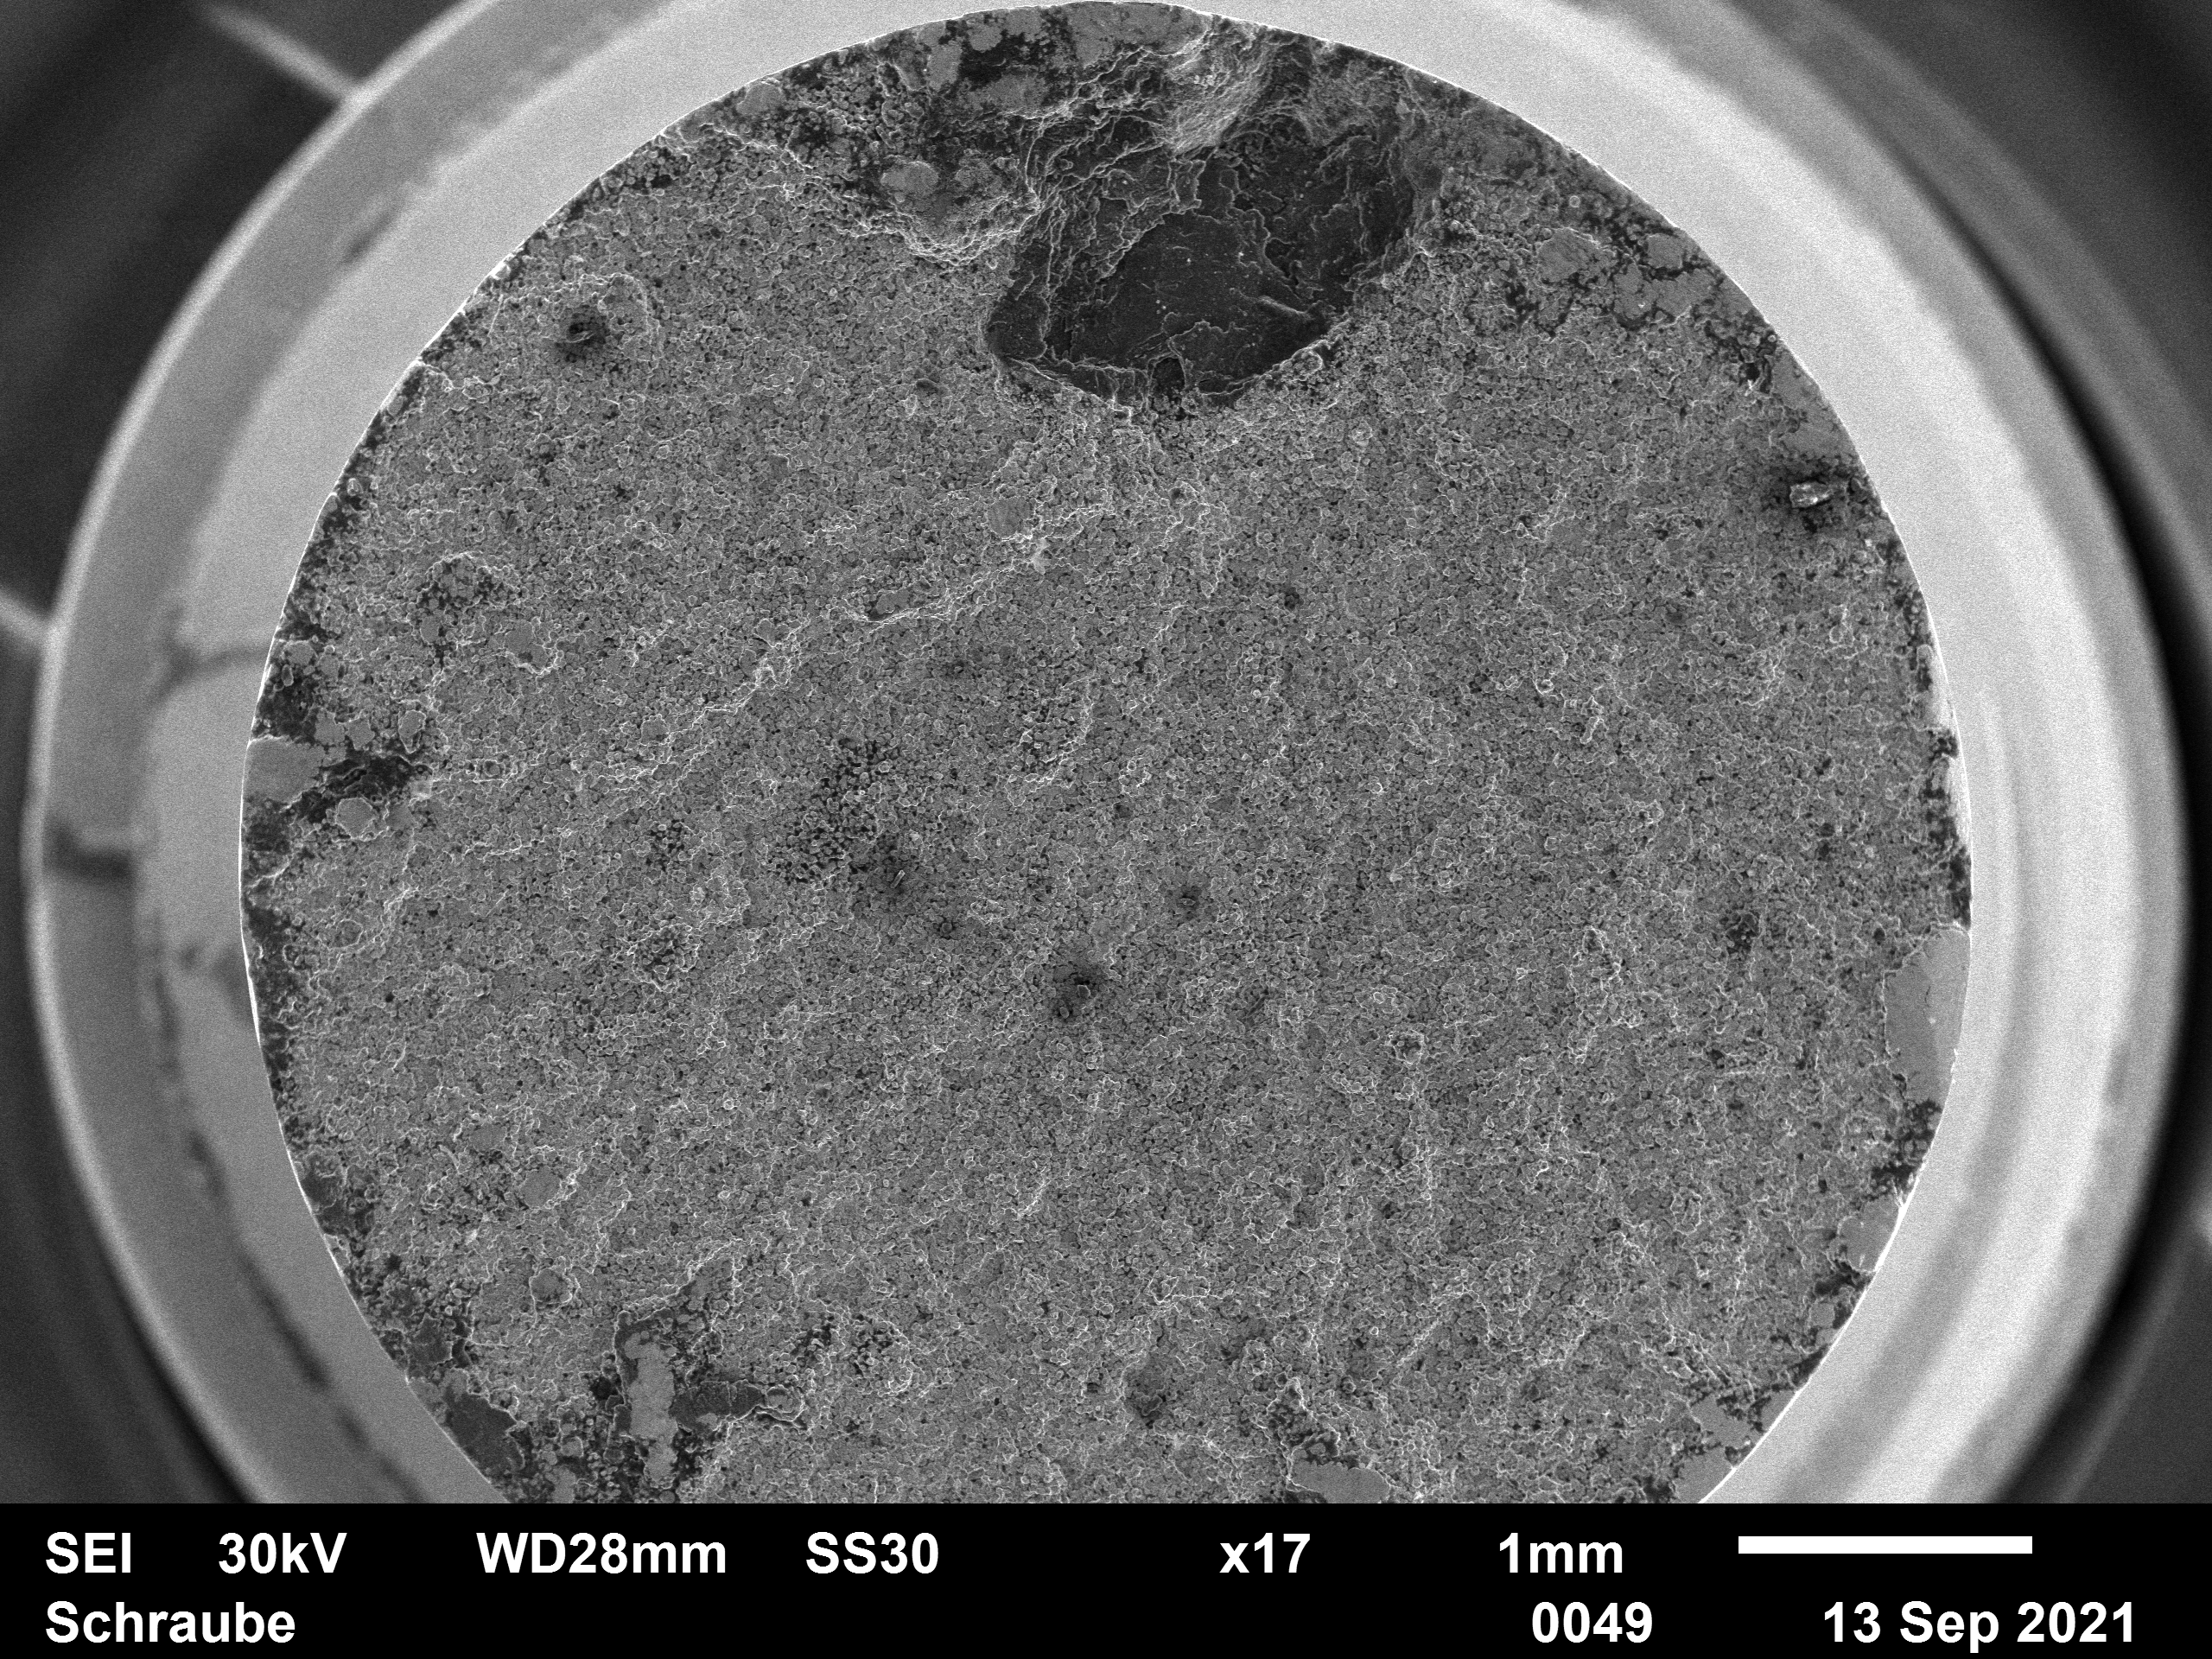
\includegraphics[width=\textwidth]{Auswertung/D/0049.png}
        \caption{SEI}
    \end{subfigure}
    \hfill
    \begin{subfigure}[b]{0.45\textwidth}
        \centering
        \includegraphics[width=\textwidth]{Auswertung/D/0048.png}
        \caption{REF}
    \end{subfigure}
    \\
    \begin{subfigure}[b]{0.45\textwidth}
        \centering
        \includegraphics[width=\textwidth]{Auswertung/D/0047.png}
        \caption{BEC}
    \end{subfigure}
    \caption{Bruchfläche der Schraube mit unterschiedlichen Detektoren}
\end{figure}
Für einen ersten Eindruck wurde der SEI Modus verwendet, um die Struktur der Fläche zu untersuchen, wurde der REF Modus verwendet. In allen Aufnahmen und besonders im letzten Bild, im BEC Modus, sind drei unterschiedliche Zonen, bzgl. der Helligkeit, zu erkennen. Zum Einen ein recht auffälliger dunkler Fleck im oberen Teil, daneben mehrere kleine hellere Zonen, die sich am Rand der Fläche zu konzentrieren und der übrige Teil der Schraube, dessen Helligkeit zwischen den beiden anderen Zonen liegt. \\

\newpage
Als Nächstes wurde eine Nahaufnahme des dunklen Flecks angefertigt.
\begin{figure}[h]
    \centering
    
    \begin{subfigure}[b]{0.45\textwidth}
        \centering
        \includegraphics[width=\textwidth]{Auswertung/D/0050.png}
        \caption{SEI}
    \end{subfigure}
    \hfill
    \begin{subfigure}[b]{0.45\textwidth}
        \centering
        \includegraphics[width=\textwidth]{Auswertung/D/0051.png}
        \caption{REF}
    \end{subfigure}
    \caption{Nahaufnahme der Kante des dunklen Flecks}
\end{figure}

Aus diesen Aufnahmen geht hervor, dass der dunkle Fleck mit einer Vertiefung einhergeht, was durch den Schatten im REF Bild zu erkennen ist. Außerdem unterscheidet sich die Textur deutlich. Im dunklen Bereich gibt es mehr ebene Flächen, wohingegen der hellere Bereich deutlich rauer ist. Das lässt darauf schließen, dass sich im dunklen Bereich eine Verunreinigung evtl. ein Fremdpartikel befand.

\newpage
Nun soll eine EDX Analyse über die Materialzusammensetzung des dunklen Flecks Aufschluss geben.
\begin{figure}[h]
    \centering
    \includegraphics[width=\textwidth]{Auswertung/D/DunkelEDX.png}
    \caption{Röntgenspektrum des dunklen Flecks}
\end{figure}


\begin{table}[h]
    \centering
    \begin{tabular}{c|c|c|c|c|c|c}
        Element & OZ &Serie& unn. C & norm. C &  Atom. C  & Fehler (1 Sigma) \\
         & & & [Gew. \%] & [Gew. \%] & [At. \%] & [Gew. \%] \\
        \hline\hline
        C & 6 & K & 56,69 & 43,02 & 55,43 & 14,77\\
        O & 8 & K & 41,46 & 31,46 & 30,43 & 10,20\\
        Na & 11 & K & 0,89 & 0,67 & 0,45 & 0,16\\
        Si & 14 & K & 32,74 & 24,85 & 13,69 & 1,56
    \end{tabular}
    \caption{Ergebnisse der EDX-Analyse des dunklen Bereichs}
\end{table}
Es fällt auf, dass kein Metall, welches in Schrauben üblicherweise verwendet wird, gefunden wurde. Dies bekräftigt die Theorie, nach welche der dunkle Fleck durch eine Verunreinigung entstanden ist.

\newpage
Des Weiteren zeigt eine Nahaufnahme der hellen Gegenden, dass sich diese durch eine gewisse Erhabenheit auszeichnen, was durch die zu erkennende Kante im Bild deutlich wird. Außerdem erscheint die Oberfläche in diesem Bereich ebener.
\begin{figure}[h]
    \centering
    \includegraphics[width=\textwidth]{Auswertung/D/0055.png}
    \caption{Nahaufnahme einer hellen Region}
\end{figure}

\newpage
Über die Zusammensetzung soll wiederum eine EDX Analyse Aufschluss geben.
\begin{figure}[h]
    \centering
    \includegraphics[width=\textwidth]{Auswertung/D/HellEDX.png}
    \caption{Röntgenspektrum der hellen Bereiche}
\end{figure}



\begin{table}[h]
    \centering
    \begin{tabular}{c|c|c|c|c|c|c}
        Element & OZ &Serie& unn. C & norm. C &  Atom. C  & Fehler (1 Sigma) \\
         & & & [Gew. \%] & [Gew. \%] & [At. \%] & [Gew. \%] \\
        \hline\hline
        C & 6 & K & 18,02 & 16,52 & 52,93 & 5,99\\
        O & 8 & K & 14,29 & 13,10 & 31,51 & 4,47\\
        Fe & 26 & K & 0,57 & 0,53 & 0,36 & 0,08\\
        Ni & 28 & K & 1,38 & 1,27 & 0,83 & 0,12\\
        W & 74 & L & 74,81 & 68,59 & 14,36 & 2,09
    \end{tabular}
    \caption{Ergebnisse der EDX-Analyse der hellen Bereiche}
\end{table}
Hier fällt die große Menge an Wolfram und Kohlenstoff auf.

\newpage
Nicht zu vergessen ist das Grundmaterial der Schraube, auch hierbei wird wieder eine EDX Analyse benutzt.
\begin{figure}[h]
    \centering
    \includegraphics[width=\textwidth]{Auswertung/D/NormalEDX.png}
    \caption{Röntgenspektrum der normalen Bereiche}
\end{figure}


\begin{table}[h]
    \centering
    \begin{tabular}{c|c|c|c|c|c|c}
        Element & OZ &Serie& unn. C & norm. C &  Atom. C  & Fehler (1 Sigma) \\
         & & & [Gew. \%] & [Gew. \%] & [At. \%] & [Gew. \%] \\
        \hline\hline
        C & 6 & K & 42,64 & 43,61 & 78,17 & 9,71\\
        O & 8 & K & 9,86 & 10,08 & 13,57 & 3,42\\
        Fe & 26 & K & 3,94 & 4,03 & 1,55 & 0,20\\
        Ni & 28 & K & 6,88 & 7,04 & 2,58 & 0,28\\
        W & 74 & L & 34,45 & 35,24 & 4,13 & 1,08
    \end{tabular}
    \caption{Ergebnisse der EDX-Analyse der normalen Bereiche}
\end{table}

Unter Berücksichtigung der soeben erlangten Erkenntnisse erscheint es als wahrscheinlich, dass der Dunkle Fleck eine Verunreinigung ist, welche bei der Herstellung in die Schmelze gelang. Diese Vermutung wurde am deutlichsten durch die EDX Analyse bestätigt, da dieser Bereich eine völlig andere Materialzusammensetzung(kaum Metalle; Sondern viel Silizium) besitzt. Die "normalen" und hellen Bereiche setzen sich hingegen aus den gleichen Materialien zusammen. \\

Durch die Verunreinigung (dunkle Anomalie) würde somit die Querschnittsfläche der Legierung an dieser Stelle verkleinert. Dies führte deshalb zu einer verminderung der stabilität, weshalb die Schraube an dieser Stelle gebrochen ist.

\newpage
\section{Chip Wafer}

Im letzten Teil haben wir uns einen Teil eines Chip Wafers vorgenommen.

\begin{figure}[h]
    \centering
    
    \begin{subfigure}[b]{0.45\textwidth}
        \centering
        \includegraphics[width=\textwidth]{Auswertung/E/0056.png}
        \caption{Großaufnahme}
    \end{subfigure}
    \hfill
    \begin{subfigure}[b]{0.45\textwidth}
        \centering
        \includegraphics[width=\textwidth]{Auswertung/E/0058.png}
        \caption{Leiterbahnen}
    \end{subfigure}
    \\
    \begin{subfigure}[b]{0.45\textwidth}
        \centering
        \includegraphics[width=\textwidth]{Auswertung/E/0061.png}
        \caption{Leiterbahnen}
    \end{subfigure}
    \hfill
    \begin{subfigure}[b]{0.45\textwidth}
        \centering
        \includegraphics[width=\textwidth]{Auswertung/E/0063.png}
        \caption{Logo}
    \end{subfigure}
    \caption{Bilder des Wafers}
\end{figure}
Gut zu erkennen sind die Leiterbahnen. Außerdem konnten wir auch ein Logo finden, wir vermuten es soll ein Mammut darstellen.

    % 5.Kapitel Fazit
    
\chapter{Fazit}
In diesem Versuch haben wir uns eingehend mit dem physikalischen System Laser befasst.
Das besondere an diesen Versuch war, dass wir hier zum ersten Mal einen Laser justieren mussten, bevor wir mit ihm Messung durchführen konnten.
Des Weiteren haben wir den Umgang mit optischen Bauelementen, dem Fabry-Perot-Interferometer und einer CCD-Kamera erlernt und trainiert. Vor allem das Justieren der optischen Bauelemente sowie das Einstellen der Spiegel war von großem Nutzen, diese Fähigkeit werden wir noch häufiger im Laufe des Praktikums benötigen.
Das außergewöhnlichste und spannendste an diesem Versuch war der Teil mit der Holografie, diese wurde hier erstmalig besprochen und untersucht.\\
Betreffend der Auswertung gab es jedoch wenig überraschendes. Die meisten Messwerte lagen im Bereich des erwarteten, vor allem wenn man die Fehler mitberücksichtigt. Die Abweichungen kamen hauptsächlich durch die entsprechende Messmethode zustande.


    % Anhang
    % Anhang

\appendix

% Text

% Charlotte Geiger - Manuel Lippert - Leonard Schatt
% Physikalisches Praktikum

% Anhang A

\chapter{Berechnungen Fourier-Reihenkoeffizient und Effektivspannung}
\label{app:Berechnung}

\section*{Sinusschwingung}
Effektivspannung:
\begin{gather}
    U_{eff} = \sqrt{\frac{1}{T}\int^T_0 U_0^2 \sin^2\left(\frac{2\pi}{T}\right) dt} = \sqrt{\frac{U_0^2}{T} \left[\frac{t}{2} - \frac{T\sin(\frac{4\pi}{T}t)}{8\pi}\bigg \vert^T_0 \right]} = \sqrt{\frac{U_0^2}{T}\frac{T}{2}} = \frac{U_0}{\sqrt{2}}
\end{gather}

\section*{Rechteckschwingung}
$b_k$ der Fourier-Reihe:
\begin{gather}
    \begin{aligned}
        b_k &= \frac{2}{T} \int^{T}_{0} f(t)\sin(k \frac{2\pi}{T} t)dt\\
            &= \frac{2}{T} \left[ \int^{\frac{T}{2}}_{0} U_0\sin(k \frac{2\pi}{T} t)dt - \int^{T}_{\frac{T}{2}} U_0\sin(k \frac{2\pi}{T} t)dt\right]\\
            &= \frac{2}{T}\frac{U_0T}{k2\pi} \left[-\cos(k \frac{2\pi}{T} t) \bigg \vert^{\frac{T}{2}}_{0} + \cos(k \frac{2\pi}{T} t) \bigg \vert^{T}_{\frac{T}{2}} \right]\\
            &= \frac{U_0}{k\pi} \left[-\cos(k\pi)+1 + 1 - \cos(k\pi)\right]\\
            &= \frac{2U_0}{k\pi}\left[1-\cos(k\pi)\right]
    \end{aligned}\\[0,5cm]
    \Rightarrow b_k =
    \begin{cases}
        0, & k~\text{gerade}\\
        \frac{4U_0}{\pi}\frac{1}{k}, & k~\text{ungerade}\\
    \end{cases}
\end{gather}

Effektivspannung:
\begin{gather}
    U_{eff} = \sqrt{\frac{1}{T}\left[\int^{\frac{T}{2}}_0 U_0^2dt + \int^T_{\frac{T}{2}} U_0^2 dt\right]} = \sqrt{\frac{U_0^2}{T}\left[\frac{T}{2}+T-\frac{T}{2}\right]} = U_0
\end{gather}

\section*{Dreiecksschwingung}
$b_k$ der Fourier-Reihe:
\begin{gather}
    \begin{aligned}
        b_k &= \frac{2}{T} \int^{\frac{3T}{4}}_{-\frac{T}{4}} f(t)\sin(k \frac{2\pi}{T} t)dt\\
            &= \frac{2}{T} \left[\int^{\frac{T}{4}}_{-\frac{T}{4}} at\sin(k \frac{2\pi}{T} t)dt+ \int^{\frac{3T}{4}}_{\frac{T}{4}} a\left(\frac{T}{2}-t\right)\sin(k \frac{2\pi}{T} t)dt\right]\\
            &= \frac{2a}{T} \left[\int^{\frac{T}{4}}_{-\frac{T}{4}} t\sin(k \frac{2\pi}{T} t)dt - \int^{\frac{3T}{4}}_{\frac{T}{4}}t\sin(k \frac{2\pi}{T} t)dt\right] + \int^{\frac{3T}{4}}_{\frac{T}{4}}a\sin(k \frac{2\pi}{T} t)dt\\
            &= (\text{I}) + (\text{II})\\[0,5cm]
        (\text{I}) &= \frac{2a}{T} \left[\int^{\frac{T}{4}}_{-\frac{T}{4}} t\sin(k \frac{2\pi}{T} t)
            dt - \int^{\frac{3T}{4}}_{\frac{T}{4}}t\sin(k \frac{2\pi}{T} t)dt\right] \Rightarrow~\text{Partielle Integration}\\
            &= \frac{2a}{T}\frac{T}{k2\pi} \left[-t\cos(k \frac{2\pi}{T} t) \bigg \vert^{\frac{T}{4}}_{-\frac{T}{4}} + t\cos(k \frac{2\pi}{T} t) \bigg \vert^{\frac{3T}{4}}_{\frac{T}{4}}\right]\\
            &\tab+\frac{2a}{T}\frac{T}{k2\pi}\left[\int^{\frac{T}{4}}_{-\frac{T}{4}} \cos(k \frac{2\pi}{T} t)dt - \int^{\frac{3T}{4}}_{\frac{T}{4}} \cos(k \frac{2\pi}{T} t)dt\right]\\
            &= \frac{2a}{T}\frac{T}{k2\pi} \left[-\frac{T}{4}\cos(k \frac{\pi}{2}) -\frac{T}{4}\cos(- k \frac{\pi}{2}) + \frac{3T}{4} \cos(k \frac{3\pi}{2}) - \frac{T}{4} \cos(k \frac{\pi}{2}) \right]\\
            &\tab+\frac{2a}{T}\frac{T}{k2\pi}\left[\int^{\frac{T}{4}}_{-\frac{T}{4}} \cos(k \frac{2\pi}{T} t)dt - \int^{\frac{3T}{4}}_{\frac{T}{4}} \cos(k \frac{2\pi}{T} t)dt\right]\\
            &= \frac{2a}{T}\frac{T}{k2\pi}\left[\int^{\frac{T}{4}}_{-\frac{T}{4}} \cos(k \frac{2\pi}{T} t)dt - \int^{\frac{3T}{4}}_{\frac{T}{4}} \cos(k \frac{2\pi}{T} t)dt\right]\\
            &= \frac{2a}{T}\left(\frac{T}{k2\pi}\right)^2 \left[\sin(k \frac{2\pi}{T} t) \bigg \vert^{\frac{T}{4}}_{-\frac{T}{4}} - \sin(k \frac{2\pi}{T} t) \bigg \vert^{\frac{3T}{4}}_{\frac{T}{2}}\right]\\
            &= \frac{2a}{T}\left(\frac{T}{k2\pi}\right)^2 \left[\sin(k\frac{\pi}{2}) - \sin(-k\frac{\pi}{2}) - \sin(k\frac{3\pi}{2}) + \sin(k\frac{\pi}{2})\right]\\[0,5cm]
        (\text{II}) &= \int^{\frac{3T}{4}}_{\frac{T}{4}}a\sin(k \frac{2\pi}{T} t)dt = \frac{aT}{2\pi} \left[\cos(k\frac{2\pi}{T}t)\bigg \vert^{\frac{3T}{4}}_{\frac{T}{4}}\right]\\
                    &= \frac{aT}{2\pi} \left[\cos(k\frac{3\pi}{2}) - \cos(k\frac{\pi}{2})\right] = 0
    \end{aligned}\\[0,5cm]
    \Rightarrow b_k =
    \begin{cases}
        0, & k~\text{gerade}\\
        \frac{8aT}{4\pi^2}\frac{(-1)^{k-1}}{k^2} = \frac{8U_0}{\pi^2}\frac{(-1)^{k-1}}{k^2}, & k~\text{ungerade}\\
    \end{cases}
\end{gather}
Effektivspannung:
\begin{gather}
    \begin{aligned}
        U_{eff} &= \sqrt{\frac{1}{T}\left[\int^{\frac{T}{4}}_{-\frac{T}{4}} (at)^2dt + \int^{\frac{3T}{4}}_{\frac{T}{4}} \left(a\left(\frac{T}{2}-t\right)\right)^2 dt\right]}\\
                &= \sqrt{\frac{a^2}{T}\left[\int^{\frac{T}{4}}_{-\frac{T}{4}} t^2dt + \int^{\frac{3T}{4}}_{\frac{T}{4}} \left(\frac{T}{2}-t\right)^2 dt\right]}
                = \sqrt{\frac{a^2}{3T}\left[t^3 \bigg \vert^{\frac{T}{4}}_{-\frac{T}{4}} - \left(\frac{T}{2}-t\right)^3 \bigg \vert^{\frac{3T}{4}}_{\frac{T}{4}}\right]}\\
                &= \sqrt{\frac{a^2}{3T}\left[\left(\frac{T}{4}\right)^3 + \left(\frac{T}{4}\right)^3 - \left(\frac{T}{2}- \frac{3T}{4} \right)^3 +  \left(\frac{T}{2}- \frac{T}{4} \right)^3\right]}\\
                &= \sqrt{\frac{a^2}{3T}\left(\frac{T^3}{16}\right)} = \sqrt{\frac{1}{3}\left(\frac{aT}{4}\right)^2} = \sqrt{\frac{U_0^2}{3}} = \frac{U_0}{\sqrt{3}}
     \end{aligned}
\end{gather}


    % Literatur
    \bibliographystyle{plainnat}
    \bibliography{Auswertung.bib}

\end{document}